\documentclass{article}%
%
%----------------------------------------------------------
% This is a sample document for the standard LaTeX Report Class
% Class options
%       --  Body text point size:
%                        10pt (default), 11pt, 12pt
%       --  Paper size:  letterpaper (8.5x11 inch, default)
%                        a4paper, a5paper, b5paper,
%                       legalpaper, executivepaper
%       --  Orientation (portrait is the default):
%                       landscape
%       --  Printside:  oneside (default), twoside
%       --  Quality:    final (default), draft
%       --  Title page: titlepage, notitlepage
%       --  Columns:    onecolumn (default), twocolumn
%       --  Start chapter on left:
%                       openright(no), openany (default)
%       --  Equation numbering (equation numbers on right is the default)
%                       leqno
%       --  Displayed equations (centered is the default)
%                       fleqn (flush left)
%       --  Open bibliography style (closed bibliography is the default)
%                       openbib
% For instance the command
%          \documentclass[a4paper,12p,leqno]{report}
% ensures that the paper size is a4, fonts are typeset at the size 12p
% and the equation numbers are on the left side.
%
\usepackage{amsmath}%
\usepackage{amsfonts}%
\usepackage{amssymb}%
\usepackage{graphicx}
\usepackage{algorithm}
\usepackage{algorithmic}
\usepackage[utf8]{inputenc} % un package pour la langue francaise
\usepackage[T1]{fontenc}      
\usepackage[francais]{babel}
%----------------------------------------------------------
\newtheorem{theorem}{Theorem}
\newtheorem{acknowledgement}[theorem]{Acknowledgement}
\newtheorem{axiom}[theorem]{Axiom}
\newtheorem{case}[theorem]{Case}
\newtheorem{claim}[theorem]{Claim}
\newtheorem{conclusion}[theorem]{Conclusion}
\newtheorem{condition}[theorem]{Condition}
\newtheorem{conjecture}[theorem]{Conjecture}
\newtheorem{corollary}[theorem]{Corollary}
\newtheorem{criterion}[theorem]{Criterion}
\newtheorem{definition}[theorem]{Definition}
\newtheorem{example}[theorem]{Example}
\newtheorem{exercise}[theorem]{Exercise}
\newtheorem{lemma}[theorem]{Lemma}
\newtheorem{notation}[theorem]{Notation}
\newtheorem{problem}[theorem]{Problem}
\newtheorem{proposition}[theorem]{Proposition}
\newtheorem{remark}[theorem]{Remark}
\newtheorem{solution}[theorem]{Solution}
\newtheorem{summary}[theorem]{Summary}

%----------------------------------------------------------
\begin{document}

\title{Métaheuristique basée sur le recuit quantique}
\author{Belaube, Bergé, Cavarec, de Méric de Bellefon, Doutre}
\date{12/05/2015}
\maketitle

\clearpage

\tableofcontents

\clearpage

\section*{Introduction}

\vspace{1cm}

Dans cet article, nous cherchons à expliquer au lecteur le principe et l'intérêt de deux métaheuristiques : le recuit simulé et son amélioration quantique. Les métaheuristiques permettent d'établir un compromis entre la résolution d'un problème difficile (un problème difficile est un problème dont la solution exacte ne peut pas être obtenue en temps polynomial) et le temps de calcul nécessaire pour le résoudre. Si ces algorithmes n'apportent pas une solution exacte au problème, ils l'apportent néanmoins rapidement et souvent avec d'excellents résultats. Nous nous sommes plus particulièrement attachés à l'étude du problème du voyageur de commerce (Traveling Salesman Problem ou TSP) mais nous souhaiterions souligner le fait que ce type d'algorithmes peut être adapté à une immense variété de problèmes difficiles.
 
			L'idée générale consiste à explorer efficacement l'espace des possibles afin d'obtenir une bonne solution. Ces algorithmes s'inspirent en particulier du chauffage suivi du refroidissement des métaux, aussi appelé recuit. Dans ce contexte, l'objectif des physiciens est de trouver l'état pour lequel l'énergie potentielle du métal est minimale en évitant les minima locaux présentés par la courbe énergétique. Le recuit simulé et le recuit quantique sont donc des algorithmes à utiliser lorsque la surface de coût n'est pas de nature convexe.
	
\vspace{1cm}

Nous définirons dans un premier temps le problème TSP. Nous verrons alors le principe du recuit simulé, les notions de physique sous-jacentes et son implémentation pratique. Nous traiterons dans un second temps des nombreux apports du recuit quantique, jusqu'alors peu étudié. Enfin, nous illustrerons ces méthodes avec les résultats obtenus sur le problème TSP.
		
\clearpage


\section{Traveling Salesman Problem}

\subsection{Présentation du problème}

Le problème du voyageur de commerce est défini par un ensemble de N villes (des noeuds) séparées entre elles par un poids ou une distance $ d_{i,j} $.
L'objectif est de permettre au voyageur de commerce de trouver la route la plus courte lui permettant de visiter toutes les villes une fois tout en revenant à son point de départ. TSP trouve de nombreuses applications dans le domaine de la logistique mais aussi dans des domaines plus exotiques tels que la conception de bras robotisés, la fabrication de puces électroniques et même le séquençage de l'ADN.
	En 1972, Richard M. Karp a montré que le problème TSP était NP-complet. Il est facile de montrer que pour un problème avec N villes, il existe $ \frac{(N-1)!}{2} $ routes possibles, soit environ le nombre estimé de particules fondamentales dans l'univers pour 70 noeuds. Supprimer la contrainte d'une unique visite ne réduit pas la complexité du problème. 

\begin{figure}[h]
\begin{center}
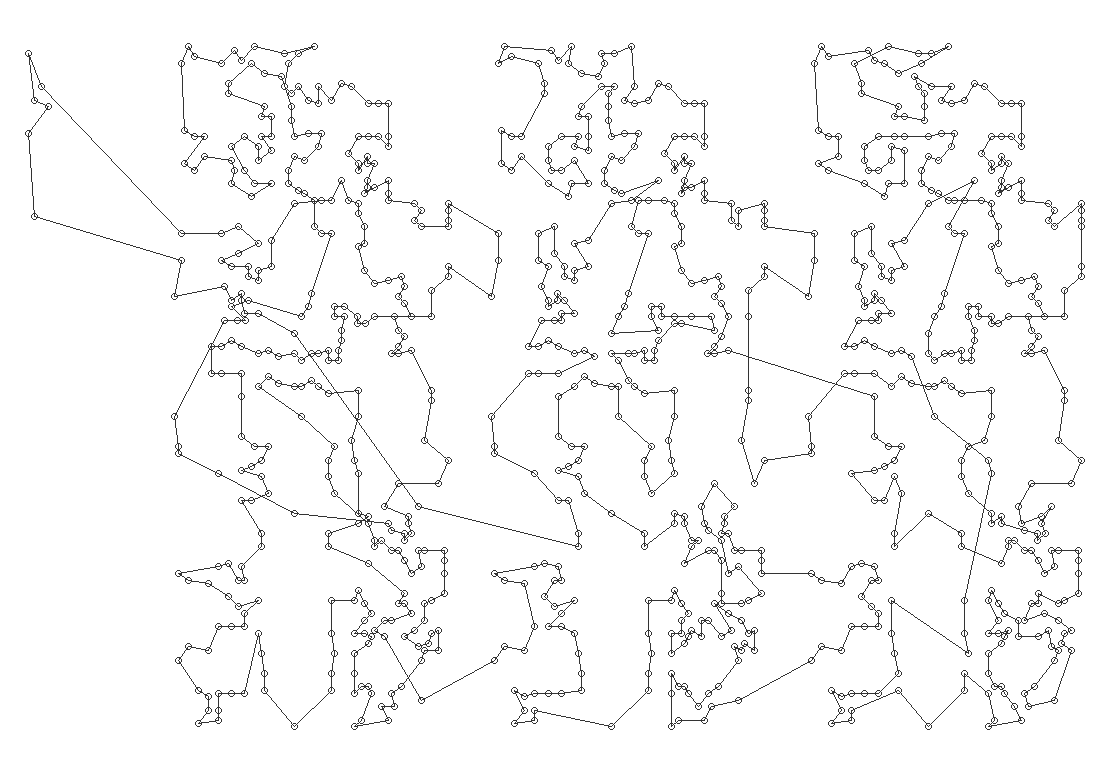
\includegraphics[scale=0.4]{pr1002.png} 
\caption{Un exemple de route solution pour le benchmark pr1002}
\end{center}
\end{figure}

Remarquons que $ d_{i,j} $ est une notion abstraite. Le graphe ne doit pas nécessairement respecter l'inégalité triangulaire ni même comporter des arêtes affectées de poids symétriques. Ces variantes ne manquent souvent pas d'accroître la nature non convexe du problème en créant de nouveaux minima locaux.

\subsection{Cartographie des minima locaux}

L’idée est de tenter d’établir une carte des minima locaux pour affiner le paramétrage. Cela fournirait également un outil supplémentaire pour comparer deux recuits différents entre eux, en comparant leur localisation dans le voisinage proche du minimum global du graphe.
Le problème est a priori complexe car il n’est pas possible de représenter en deux dimensions une carte où l’on pourrait voir une courbe continue dessinant la surface des énergies en fonction des routages. En effet, deux routages peuvent avoir un rapprochement très grand et pour autant ne pas avoir des énergies voisines, puisque l’énergie est liée au poids des arêtes et non à l’existence ou non de ces arêtes.
Ainsi, il convient d’essayer d’estimer la densité des minima locaux, en regard à une norme donnée. 
Une nouvelle difficulté apparaît : positionner les répliques les unes par rapport aux autres en peu de temps de calcul car cette cartographie est a priori en temps exponentiel. 



\begin{figure}[h]
\begin{center}
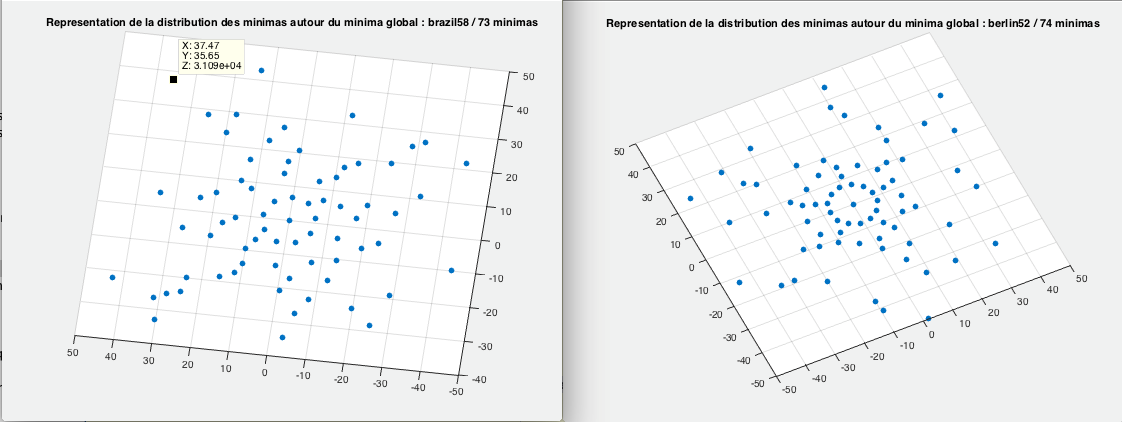
\includegraphics[scale=0.3]{cartes.png} 
\caption{Cartographie des minima locaux sur le benchmark brazil58}
\end{center}
\end{figure}


      Le lieu où la densité des minima nous intéresse est centré sur le minimum global.  On décide alors de comparer la distance des répliques correspondant à des minima locaux au minimum global seul pour diminuer le temps de calcul.
      L’idée est donc d’estimer une distance radiale d’un minimum local au minimum global, sans tenir compte a priori de la distance des minima locaux entre eux. Ainsi, chaque minimum local trouvé peut être placé une carte. On le place sur un cercle centré sur le minimum global et dont le rayon correspond à sa distance du minimum global.
      L’idée de placer chaque minimum local aléatoirement sur un cercle permet une visualisation en trois dimensions de la densité de minima, et souligne la possibilité d’intégrer une information supplémentaire dans le modèle en jouant sur l’angle aléatoire - par exemple, pour deux minima différents qui ont une distance identique au minimum global, prendre en compte la distance entre eux et en rendre compte dans leur éloignement sur leur cercle.

\clearpage

\section{Recuit Simulé}

\subsection{Principes physiques}

	C'est au début des années 80 que Kirkpatrick a généralisé la notion de recuit simulé. En métallurgie, le recuit consiste à chauffer un métal jusqu'à sa température de fusion puis à le refroidir très lentement jusqu'à ce que les atomes se réarrangent pour regagner l'état solide. L'état fondamental du solide sera atteint seulement si la température initiale est assez élevée et si le refroidissement est suffisamment lent. Si ces conditions ne sont pas respectées, le métal se retrouve dans un minimum local d'énergie potentielle, c'est à dire un état méta-stable.
	
	Il convient donc de jouer avec la variation de température pour permettre au système de sortir des minima locaux. En 1953, Metropolis avait déjà développé un algorithme recréant l'évolution d'un métal au cours du recuit. En partant d'un état dont l'énergie est égale à $E_i$, on applique une légère variation de température. À l'équilibre thermique, le système peut se retrouver dans un état j dont l'énergie est $E_j$.
	
	La probabilité qu'un solide soit dans un état i avec une énergie $E_i$ à la température T est donnée par : $\mathbb{P}$(\emph{X}=i) = $e^{\frac{-E_i}{k_BT}} / \sum_{j=0} e^{\frac{-E_j}{k_BT}}$. Plus l'énergie de l'état i est faible par rapport à celle des états j, plus le système a des chances de se retrouver dans cet état. C'est pourquoi Metropolis choisit de fixer la probabilité d'acceptation d'un passage A de l'état i à j à la température T par $\mathbb{P}$(A) = min(1,$e^\frac{(E_i-E_j)}{k_BT}$). On vérifie que cette probabilité vérifie l'équation d'équilibre de Markov. 
	
	\vspace{1cm}
	
	En faisant l'analogie entre une solution du problème et un état du système et entre l'énergie d'un état et le coût de la solution, on peut alors construire l'algorithme du recuit simulé :
	
	\begin{algorithm} 
	\caption{Recuit Simulé}
	\begin{algorithmic}
	
	\STATE $sol \leftarrow RealisationAleatoire$
	\FOR{$it=0; it < N; it++$}	
		\STATE $sol \leftarrow mutation( sol ) $
		\STATE $\Delta{E} \leftarrow E_j-E_i$
		\IF{$\Delta{E}\prec{0}$} 
			\STATE Accepter cette mutation	
		\ELSE 
			\STATE Ne l'accepter qu'avec une probabilité égale à $\mathbb{P}$(A)
		\ENDIF
		\STATE Choisir $T_{k+1}$ plus petit que $T_{k}$
	\ENDFOR
	\RETURN $sol$
	\end{algorithmic}
	\end{algorithm}
\vspace{1cm}

Ainsi, aux hautes températures, le système change d'état quasiment aléatoirement. Il explore la surface d'énergie de manière globale. Lorsque la température décroit, le système a de moins en moins de chance d'accepter de passer dans un état qui augmente son énergie. La recherche d'une solution devient alors locale car l'état courant ne peut plus franchir une barrière d'énergie importante. Plus le refroidissement est lent, plus le système a de chances d'atteindre un état dont l'énergie est proche de l'énergie fondamentale. Le lecteur attentif aura compris que les éléments importants du recuit simulé sont : la température initiale, le taux de décroissance de la température à chaque itération et enfin la nature de la mutation élémentaire. $K_B$ est arbitrairement fixé égal à 1.

Dans la section suivante, nous montrerons comment nous sommes parvenus à fixer les paramètres importants du recuit.

\subsection{Implémentation}

\vspace{1cm}

	Pour utiliser cet algorithme sur le problème du voyageur de commerce, il faut commencer par définir les différents éléments indispensables au recuit : l'état, l'énergie et la mutation.
	Un état est défini comme une solution possible au problème donné. Par exemple, pour le problème SAT, l'état est l'assignation d'un booléan à chaque variable. Pour le problème TSP, l'état est une route c'est-à-dire une suite d'arêtes où chaque noeud n'est traversé qu'une seule et unique fois. D'un point de vue informatique, une route sera représentée par une liste de noeuds. Le graphe est représenté par une matrice carrée des distances $ d_{i,j} $. La taille de cette matrice définit le nombre de noeuds dans la route. À chaque état est associée une énergie. Cette énergie correspondra ici à la longueur totale de la route : c'est la somme des longueurs de chacune des arêtes $ (i,j) $ de la route, chaque longueur étant donnée par la matrice du graphe.
	
	
	\begin{table}[hp]
		\centering
			\begin{tabular}{|*{5}{c|}}
					\hline
					0  & 2  & 3 & 4 & 5 \\
					\hline
					2  & 0 & 6 & 8 & 1 \\
					\hline
					3  & 6 & 0 & 3 & 5 \\
					\hline
					4  & 8 & 3 & 0 & 2 \\
					\hline
					5  & 1 & 5 & 2 & 0 \\
					\hline
			\end{tabular}
		\label{tableau_distances}
		\caption{Exemple de graphe à 5 noeuds}
	\end{table}

		Pour le graphe décrit sur le tableau~\ref{tableau_distances}, l'énergie correspondant à la route définie par les noeuds $ 0\rightarrow 2\rightarrow 4\rightarrow 1\rightarrow 3 $ vaut 3+5+1+8+4 donc 21. On se réfère ici à une indexation Java, commençant à 0. De plus, comme c'est le cas pour ce graphe, tous les problèmes traités dans ce document seront symétriques.
		Pour ce qui est de la mutation, nous utiliserons 2-opt car c'est la mutation sur TSP qui modifie le moins d'arêtes, à savoir 2, entre l'état courant et l'état muté. Nous démontrons en figure~\ref{mutations} que c'est la mutation la plus efficace face à des mutations qui modifient davantage d'arêtes.
		La mutation 2-opt consiste à choisir deux noeuds i et j différents de la route, à les échanger et à échanger les noeuds 'intermédiaires', autrement dit à échanger le noeud suivant i et le noeud précédent j, etc... L'implémentation de cette mutation est expliquée sur la figure ~\ref{2opt}.
	
	\begin{figure}[!h]
		
	\begin{center}
	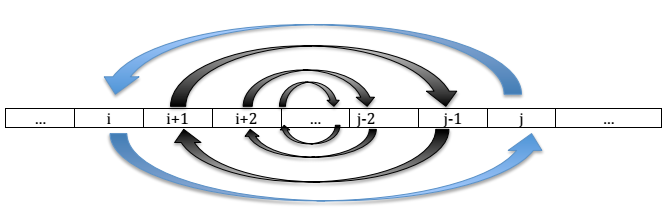
\includegraphics[scale=0.25]{2opt.png}
	\caption{Fonctionnement de la mutation 2-opt}
	\label{2opt}
	\end{center}
	\end{figure}
	
	\begin{figure}[!h]
		
	\begin{center}
	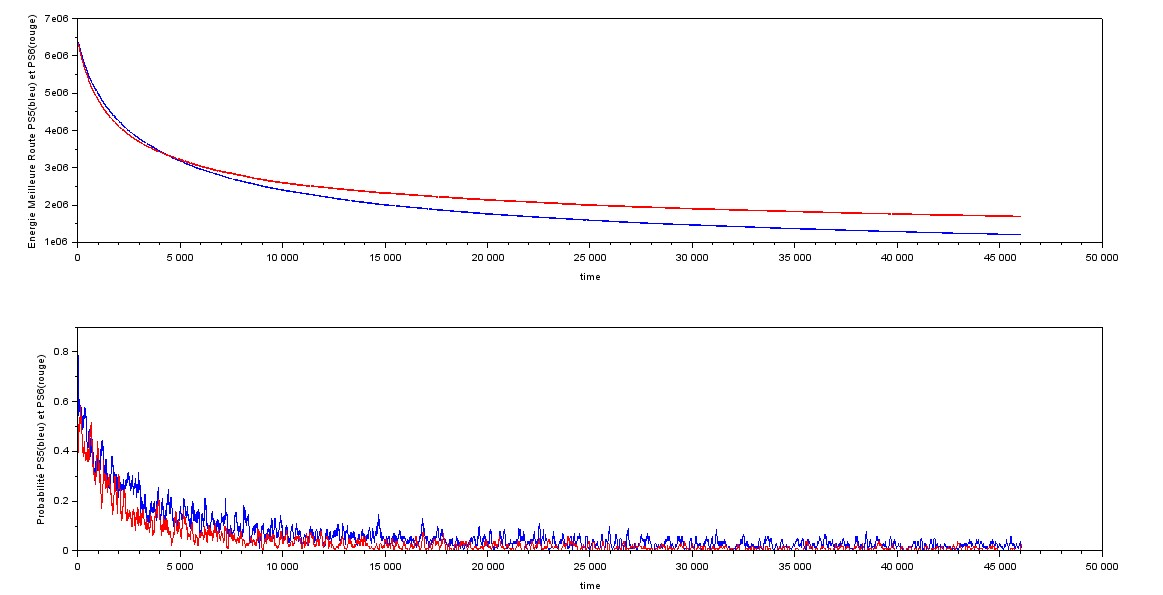
\includegraphics[scale=0.25]{pr1002_mutation.jpg}
	\caption{Comparaison entre 2-opt(en bleu) et 3-opt(en rouge)}
	\label{mutations}
	\end{center}
	\end{figure}
			
			L'étude de l'influence des paramètres est primordiale si l'on souhaite exécuter un recuit efficace. Pour un recuit simulé, étant donné que $ K_{B} $ est fixé, le seul paramètre à prendre en compte est la température. Mais ce paramètre n'est pas fixe, il décroît et il y a donc trois données à définir : la température de début $ T_{deb} $, la température de fin $T_{fin} $ et le mode de décroissance. On s'est très vite aperçu, et cela est parfaitement cohérent, que fixer une fonction température $ T_{n} $ ne donnait pas des résultats satisfaisants sur tous les benchmarks. Cette expérience est décrite dans le tableau ~\ref{perf_random_sa} où on pose $ T_{deb} = 1000 $ , décroissance exponentielle avec un facteur de décroissance de 0.99. La température de fin est très proche de 0. On a $ T_{n} = 1000 \times 0.99^{n} $ avec n = $0..100 \times 58 \times 58 $
			
	\begin{figure}[!h]
	\begin{center}
	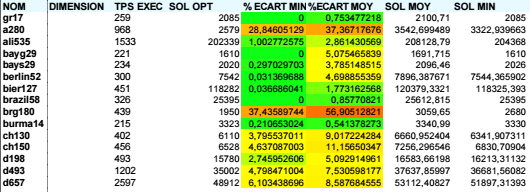
\includegraphics[scale=0.4]{perf_random_sa.png}
	\caption{Solution en énergie du recuit simulé pour une température arbitraire}
	\label{perf_random_sa}
	\end{center}
	\end{figure}
	
		En réalité, il n'existe pas de fonction température universelle, compatible avec tous les graphes. Pour utiliser correctement le recuit simulé, il faut adapter la température à chaque graphe.
		
		\vspace{1cm}
		
		On va, pour cela, essayer de trouver un algorithme qui détermine correctement la température du recuit en fonction du graphe traité : un paramétreur universel.
		Rappelons rapidement quel est le rôle de la température. Elle ajuste la valeur de la probabilité d'acceptation lorsque la mutation nous dirige vers un état plus haut en énergie : $ p = e^{-\frac{\Delta E}{KT}} $. Il faut paramétrer de telle sorte que les probabilités d'acceptation soient quasi-idéales pour une bonne utilisation du recuit. Sur une évaluation, $ p $  dépend donc de $ \Delta E $ et de $ T $. 
		Pour concevoir notre paramétreur, on va émettre deux hypothèses importantes. Tout d'abord, on émet l'hypothèse que l'efficacité du recuit simulé dans son ensemble dépend de $ T_{n} $ et de la distribution globale de toutes les différences d'énergie $ \Delta E $ engendrées par des 2-opt sur le graphe. On construira donc un échantillon trié de 1000 $ \Delta E $. Dans un second temps, on suppose qu'il existe un intervalle $ (\Delta E)_{i} \leq T_{n} \leq (\Delta E)_{j} $ de cette distribution où le recuit est efficace pour tout graphe. Autrement dit, on veut trouver i et j universels. 
		L'objectif est donc de déterminer ces deux indices désormais. Sur plusieurs benchmarks, on lance des recuits pour une décroissance linéaire, $ T_{fin} = 0 $ avec différentes températures de départ $ T_{deb} = 2.(\Delta E)_{k} $. On notera les différentes valeurs de k qui donnent les meilleurs recuits pour se faire une idée de l'intervalle [i,j].
		
	\begin{figure}[!h]
	\begin{center}
	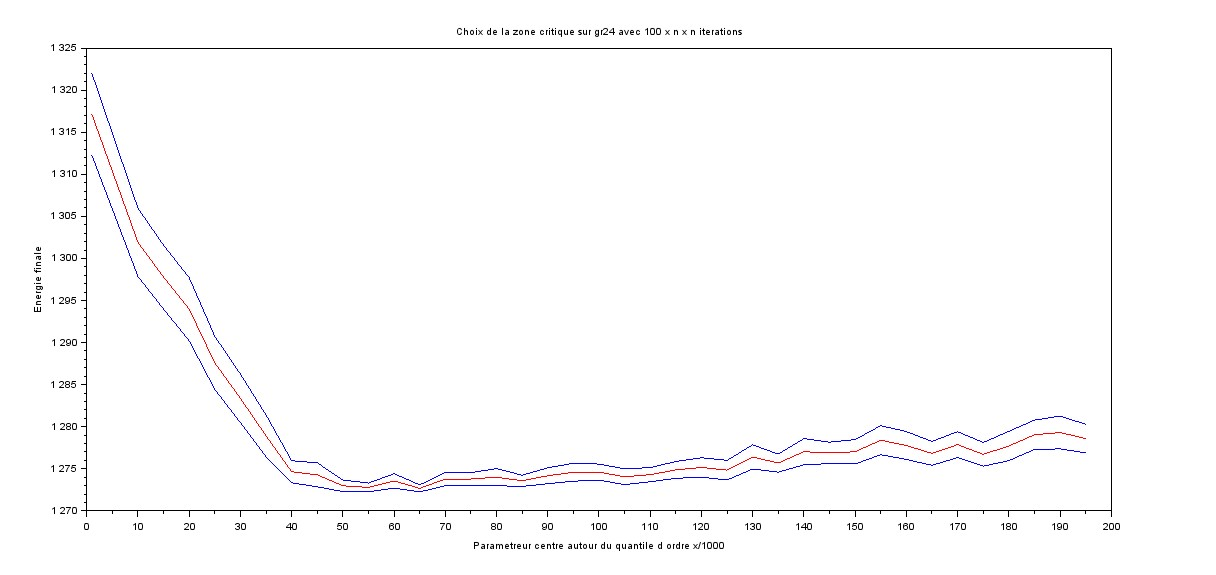
\includegraphics[scale=0.25]{gr24_zonecritique.jpg}
	\caption{Performance du recuit pour $ T_{deb} = 2. (\Delta E)_{k} $ sur gr24}
	\label{gr24_zone}
	\end{center}
	\end{figure}
	
	\begin{figure}[!h]
	\begin{center}
	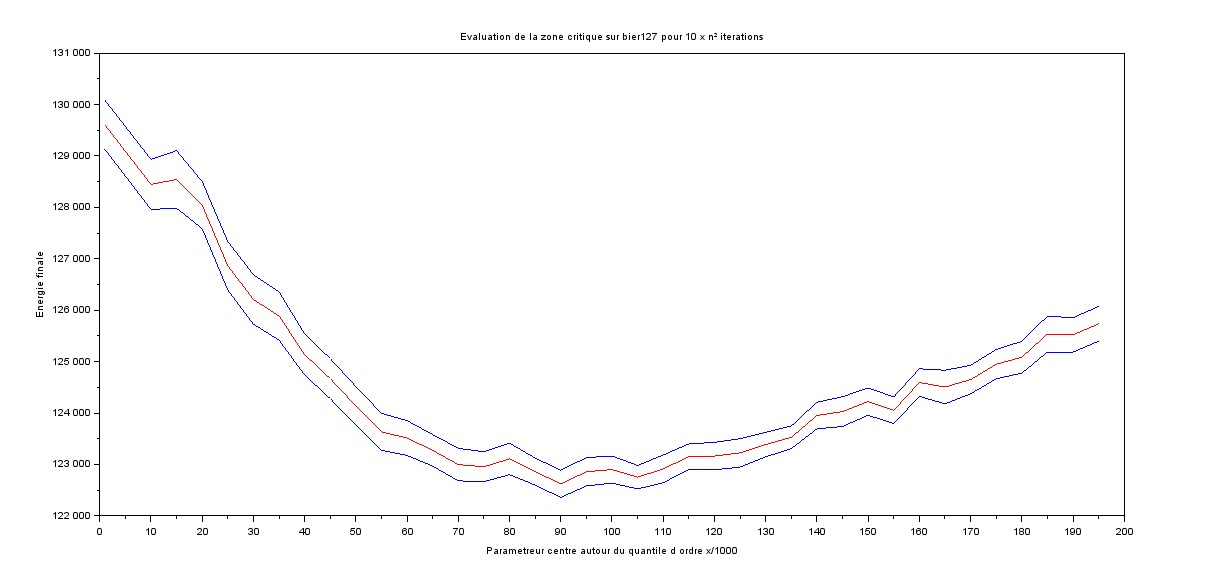
\includegraphics[scale=0.25]{bier127_zonecritique.jpg}
	\caption{Performance du recuit pour $ T_{deb} = 2. (\Delta E)_{k} $ sur bier127}
	\label{bier127_zone}
	\end{center}
	\end{figure}
	
	\begin{figure}[!h]
	\begin{center}
	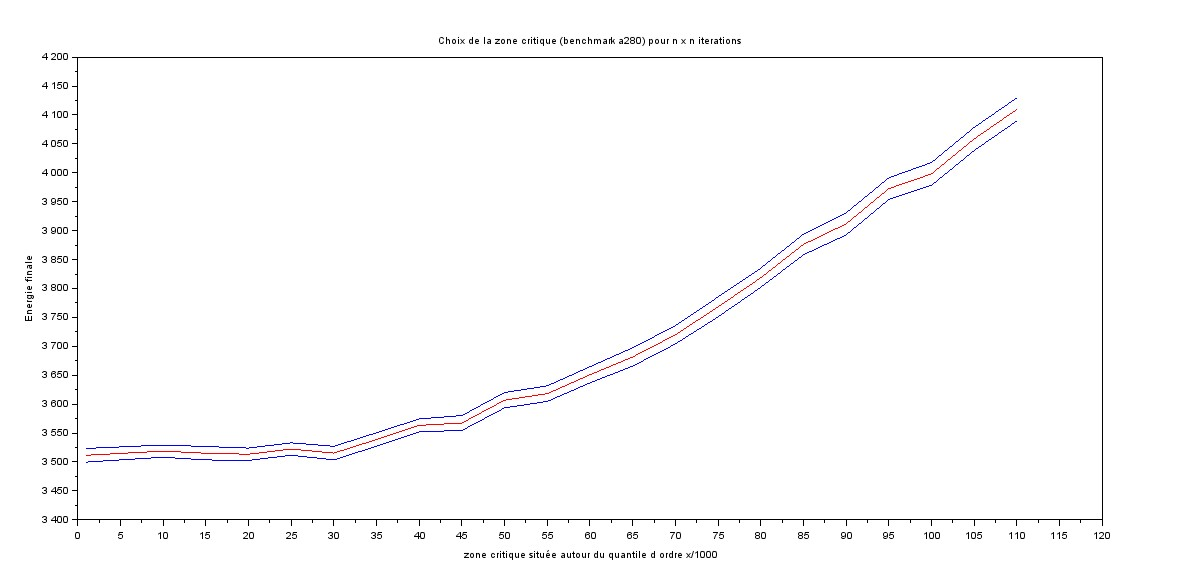
\includegraphics[scale=0.25]{a280_zonecritique.jpg}
	\caption{Performance du recuit pour $ T_{deb} = 2. (\Delta E)_{k} $ sur a280}
	\label{a280_zone}
	\end{center}
	\end{figure}
		
		Les trois figures précédentes présentent les résultats de cette expérience sur plusieurs exemples. On constate que sur chacune d'entre elles, la zone $ 2. (\Delta E)_{50} \leq T_{deb} \leq 2. (\Delta E)_{100} $ fournit les meilleurs résultats. Il faut donc concentrer la température autour du cinquième centile et du premier décile de la distribution des $ \Delta E $.
		Pour une décroissance linéaire, on posera $ T_{deb} = (\Delta E)_{100} $ et $ T_{fin} = (\Delta E)_{50} $. 
		Pour une décroissance exponentielle, on posera $ T_{deb} = 10.(\Delta E)_{100} $ et $ T_{fin} = (\Delta E)_{50} $.
		
	\begin{figure}[!h]
	\begin{center}
	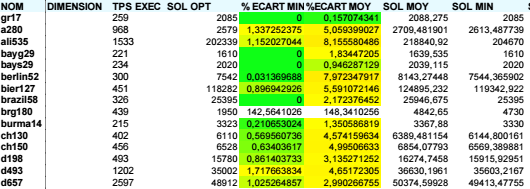
\includegraphics[scale=0.4]{perf_lin.png}
	\caption{Performance du recuit avec le paramétreur en décroissance linéaire}
	\label{perf_lin}
	\end{center}
	\end{figure}
	
	\begin{figure}[!h]
	\begin{center}
	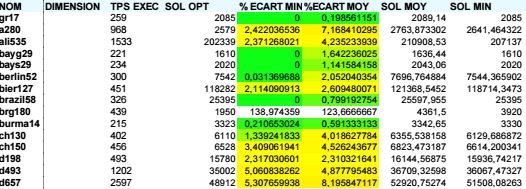
\includegraphics[scale=0.4]{perf_exp.png}
	\caption{Performance du recuit avec le paramétreur en décroissance exponentielle}
	\label{perf_exp}
	\end{center}
	\end{figure}
	
	Les figures ~\ref{perf_lin} et ~\ref{perf_exp} nous fournissent les performances de notre paramétreur sur un lot d'une quinzaine de benchmarks en $100n^2 $ itérations. Si l'on compare avec la figure ~\ref{perf_random_sa}, le pourcentage moyen est clairement amélioré. Seul le graphe brg180 résiste à notre paramétreur : en regardant la matrice des distances de ce benchmark, on s'aperçoit qu'elle est assez particulière : les énergies des arêtes sont très similaires, certaines sont infinies,... Cela crée des discontinuités importantes dans la distribution des $ \Delta E $ et le paramétreur prend souvent une valeur trop élevée pour T sur tout le recuit. A noter que non seulement brg180 se résoud très bien avec T = 0 mais aussi que de telles discontinuités ne peuvent apparaître avec un graphe euclidien.
	
	\begin{algorithm}[!h] 
	\caption{Paramétreur linéaire}
	\begin{algorithmic}
	
	\STATE $ l \leftarrow{listeVide} $
	\FOR{$ k = 0; k < 1000; k++ $}
		\STATE $ r \leftarrow{new RouteAleatoire} $
		\STATE $r \leftarrow mutation( r ) $
		\STATE $\Delta{E} \leftarrow E_j-E_i$
		\IF{$\Delta{E} > 0$}
			\STATE{$l.ajoute(\Delta{E})$}
		\ENDIF
	\ENDFOR
	\STATE{$l.trie()$}
	\STATE{$ T_{deb} = l.get(100) $}
	\STATE{$ T_{fin} = l.get(50) $}
	\STATE{$ coefficientDeRefroidissement = \frac{T_{fin}-T_{deb}}{N} $}
	\end{algorithmic}
	\end{algorithm}
	
	L'application du recuit simulé sur TSP pose le problème des paramètres. La recherche de la bonne température pour un seul graphe nécessite déjà de nombreux tests. Nous avons proposé à l'utilisateur une méthode permettant de calibrer automatiquement la température. Cette méthode ne correspond bien évidemment pas au paramétrage idéal. Cependant, si le temps nous est compté, elle évite des tests encombrants pour trouver T et donne une bonne approximation du minimum global de notre problème. Le temps d'exécution du paramétreur est négligeable comparé à celui du recuit simulé qui ne dépasse jamais quelques secondes pour des graphes de moins de 1000 noeuds traités en plusieurs millions d'évaluations.
	
	
\clearpage
\section{Recuit Quantique}
\subsection{Fonctionnement}

	\vspace{1cm}
	
	Le recuit quantique est une méta-heuristique qui approfondit le modèle du recuit simulé. Il nous faut d'abord évoquer ce qu'on pourrait appeler un recuit simulé 'en parallèle' ou SA parallèle qui, au lieu de travailler sur un seul état, traiterait plusieurs états en même temps. On aurait alors le choix entre appliquer, sur un problème, un recuit simulé pour $ 10.n^2 $ itérations ou un recuit parallèle de 10 répliques, chacune en $ n^2 $ itérations. On appelle particule l'ensemble de ces 10 répliques. L'avantage du SA parallèle est de dompter, plus que ce que fait le SA classique, le côté combinatoire de ces heuristiques. Par exemple, s'il existe un graphe avec 10 minimums locaux profonds en énergie, le SA classique va se bloquer dans l'un de ces minima alors que le SA parallèle va en explorer plusieurs. Par contre, la décroissance en moyenne du SA parallèle en énergie est plus lente que pour un recuit simulé classique.
	Le recuit quantique ou QA est un SA en parallèle dont l'hamiltonien a deux composantes : potentielle et cinétique. La composante cinétique est calculée à partir des matrices de spins des états de la particule. Pour TSP, la matrice de spin notée S d'une route est une matrice triangulaire supérieure. Pour $ i < j $, on ajoute 1 aux indices (i,j) si l'arête correspondante appartient à la route, -1 sinon. La diagonale est constituée de zéros. 
	
	\begin{table}[hp]
		\centering
			\begin{tabular}{|*{5}{c|}}
					\hline
					0  & 1  & -1 & -1 & 1 \\
					\hline
					0  & 0 & -1 & 1 & -1 \\
					\hline
					0  & 0 & 0 & 1 & 1 \\
					\hline
					0  & 0 & 0 & 0 & -1 \\
					\hline
					0  & 0 & 0 & 0 & 0 \\
					\hline
			\end{tabular}
		\label{spin}
		\caption{Matrice de spin de la route $ 0 \rightarrow 1 \rightarrow 3 \rightarrow 2 \rightarrow 4 $}
	\end{table}
	
	Les répliques sont agencées sous forme de chaînage ou de liste en début de recuit. Ainsi, une réplique a deux répliques voisines fixes tout au long de l'algorithme. L'énergie cinétique est proportionnelle aux produits scalaires des matrices de spin entre routes voisines. On a alors $ H_{cin} = J_{\Gamma}.(\sum_{k=1}^(P-1) \sum_{i<j} S_{(i,j),k}.S_{(i,j),k+1} + S_{(i,j),P}.S_{(i,j),1})$ où $ P $ est le nombre de répliques. $ \Gamma $ est un paramètre semblable à $ T $ dans la mesure où il faudra savoir définir $ \Gamma_{deb} $ , $ \Gamma_{fin} $ et le mode de décroissance. On utilisera l'expression suivante pour déterminer $ J_{\Gamma} $ : $ J_{\Gamma} = -0.5T.ln(tanh(-\frac{\Gamma}{PT})) $. 
		L'objectif du recuit quantique est donc de minimiser l'hamiltonien $ H = H_{pot} + H_{cin} = \frac{1}{P}.\sum_{k=0}^P H_{pot,k} + H_{cin} $.
		
	\begin{algorithm}[!h] 
	\caption{Recuit Quantique}
	\begin{algorithmic}
	
	\STATE $p \leftarrow creeParticule$
	\FOR{$it=0; it < N; it++$}	
		\FOR{$k=1; k \leq P; k++$}
			\STATE $sol \leftarrow p.getReplique(k) $
			\STATE $sol \leftarrow mutation( sol ) $
			\STATE $\Delta{E} \leftarrow E_j-E_i+\Delta{E_{cin}}$
			\IF{$\Delta{E}\prec{0}$} 
				\STATE Accepter cette mutation	
			\ELSE 
				\STATE Ne l'accepter qu'avec une probabilité égale à $\mathbb{P}$(A)
			\ENDIF
			\STATE Choisir $T_{k+1}$ plus petit que $T_{k}$
			\STATE Choisir $\Gamma_{k+1}$ plus petit que $\Gamma_{k}$
			\STATE Modifier l'ordre de parcours des répliques sans modifier le chaînage
		\ENDFOR
	\ENDFOR
	\STATE $ bestSol \leftarrow p.getMeilleureReplique $
	\RETURN $ bestSol $
	
	\end{algorithmic}
	\end{algorithm}
		
		\vspace{1cm}

\subsection{Réglages et paramètres}

\vspace{1cm}

	Le réglage de la température se fait avec le paramétreur présenté dans le chapitre 'Recuit Simulé'. On pose $ T = \Delta E_{50} $ (cinquième centile de la distribution des $ \Delta E $)
	Un facteur important à régler est le nombre de répliques à utiliser. Le nombre de répliques idéal dépend du nombre de noeuds du graphe que l'on traite et du nombre d'itérations. Traiter un graphe de 100 noeuds en $ 10.n^2 $ ne nécessite pas d'employer le même nombre de répliques qu'avec $ 100.n^2 $. On effectue cette expérience sur un graphe de 52 noeuds : on trace le résultat en fonction du nombre de répliques pour différentes valeurs du nombre d'itérations sur la figure ~\ref{berlin52_nbRepliques}. Pour la courbe bleue, le nombre de répliques idéal est 1. En revanche, lorsque le nombre d'évaluations augmente (courbe noire), le nombre de répliques idéal est proche de 10.
	
	\begin{figure}[!h]
	\begin{center}
	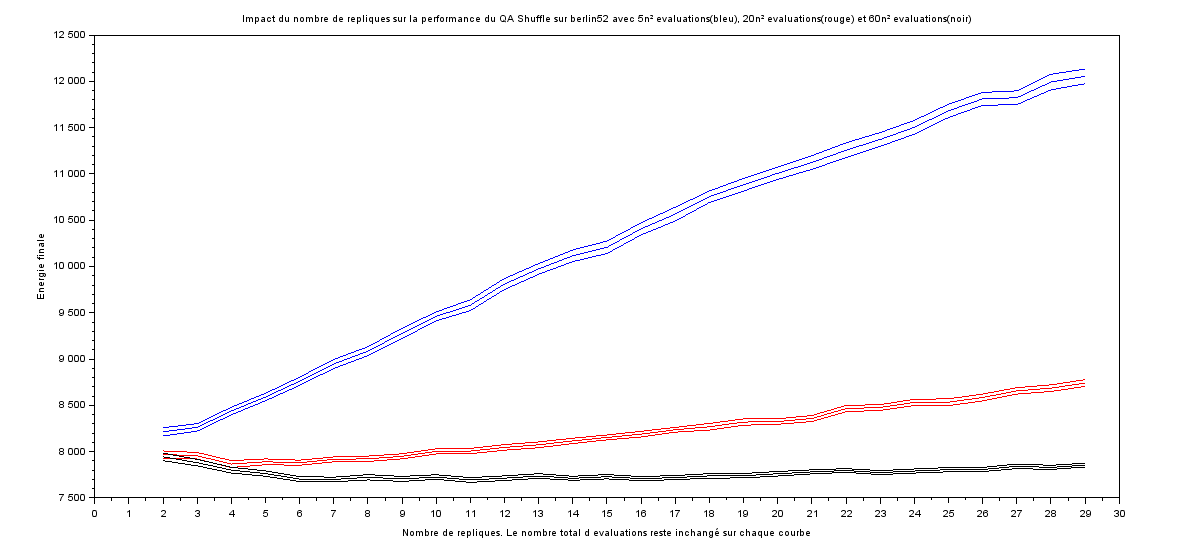
\includegraphics[scale=0.25]{berlin52_nbRepliques.png}
	\caption{Performance du recuit quantique en fonction de P en $ 5n^2 $ (bleu) , $ 20n^2 $ (rouge) et $ 60n^2 $ (noir)}
	\label{berlin52_nbRepliques}
	\end{center}
	\end{figure}
	
	\vspace{1cm}
	
	Le dernier paramètre auquel il faut s'intéresser est $ \Gamma $. Nous avons décidé de paramétrer universellement $ \Gamma $ comme nous l'avons fait avec $ T $. La méthode est assez similaire : on va déterminer sa valeur en fonction de l'échantillon des $ \Delta E $ engendrés par des 2-opt. On suppose qu'il existe un k universel idéal tel que $ \Delta E_{cin} = \frac{(\Delta E)_{k}}{P} $ en fin de recuit où $ (\Delta E)_{k} $ est un élément de l'échantillon. La variation élémentaire de $ \Delta E_{cin} $ vaut $ 4J_{\Gamma} $ : le terme 4 provient du fait que, lors de la modification d'une arête, chaque route a deux voisins et les valeurs de spin passent de +1 à -1. On obtient donc la relation : $ J_{\Gamma_{fin}} = \frac{(\Delta E)_{k}}{4P} $. Cette relation est valable pour la dernière itération du QA. On en déduira donc $ \Gamma_{fin} $. On pose arbitrairement $ \Gamma_{deb} = 100\Gamma_{fin} $. 
	On détermine la valeur de k à l'aide d'expériences sur différents benchmarks. Comme l'illustre la figure ~\ref{gamma}, la valeur k = 200 convient parfaitement. A noter que le paramétrage de $ \Gamma $ est bien moins important que celui de T : ici, l'énergie varie seulement de quelques unités pour les différents paramétrages.
	
	\begin{figure}[!h]
	\begin{center}
	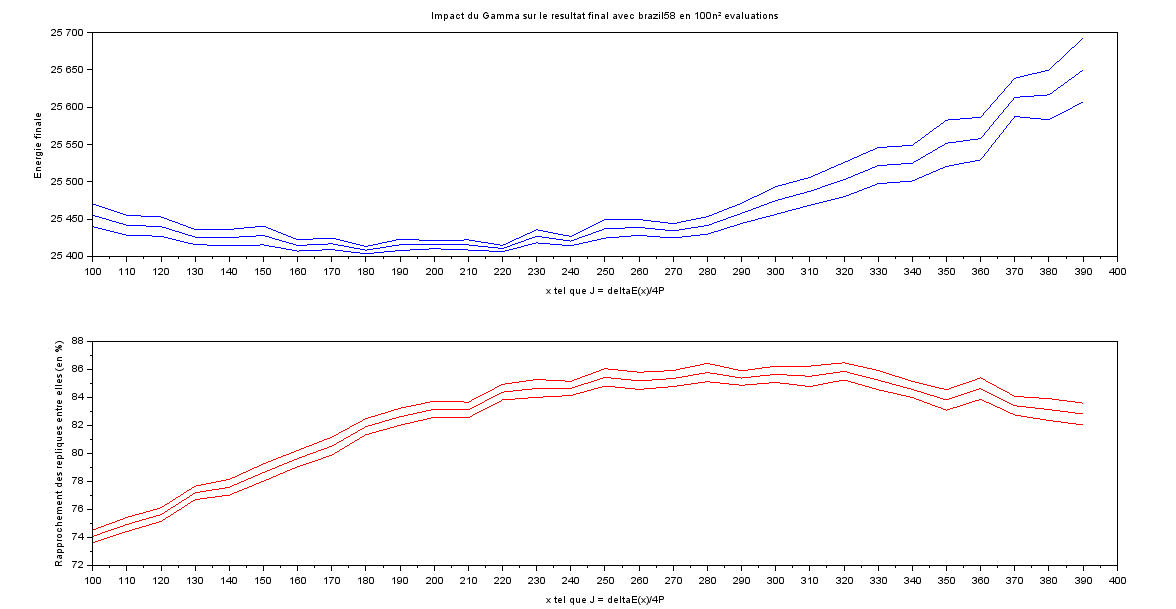
\includegraphics[scale=0.25]{gamma.png}
	\caption{Performance du recuit quantique en fonction de $ J_{fin} $}
	\label{gamma}
	\end{center}
	\end{figure}


\clearpage
\section{Résultats}

\vspace{1cm}

		Il s'agira, dans cette partie, de comparer les performances des deux algorithmes présentés précédemment. Dire lequel des deux algorithmes est le meilleur n'est pas une tâche aisée : pour certains paramètres, sur un certain graphe, le recuit simulé donne de meilleurs résultats que le recuit quantique sur un même nombre d'évaluations global. Par exemple, lorsque le nombre de répliques est extravagant sur le recuit quantique, on descend très lentement en énergie, contrairement au recuit simulé qui se rapproche rapidement du minimum global. Inversement, le recuit quantique peut être préférable dans d'autres dispositions. Il faudra donc faire attention à comparer "le meilleur recuit simulé"' au "`meilleur recuit quantique"' pour un même nombre d'évaluations.
		
\vspace{1cm}

		On traitera d'abord le comportement global des deux recuits. Un premier constat est celui concernant la valeur de l'énergie potentielle tout au long du recuit. A travers la figure suivante, on remarque que les deux algorithmes adoptent des attitudes globalement différentes.
		
	\begin{figure}[h]
	\begin{center}
	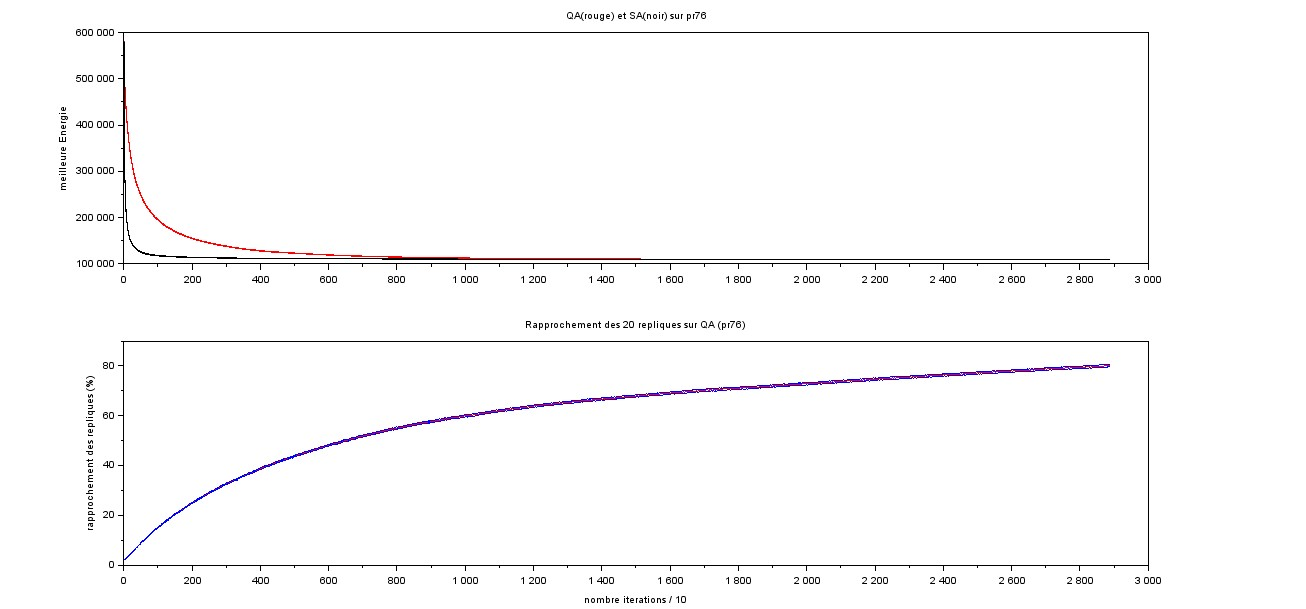
\includegraphics[scale=0.25]{comparaison_pr76.jpg}
	\caption{Evolution des énergies sur pr76 et rapprochement des répliques pour QA}
	\label{QASA}
	\end{center}
	\end{figure}
		
		Comme on peut le voir, la décroissance du recuit quantique en énergie est plus lente. D'ailleurs, plus le nombre de répliques est important, plus cette décroissance sera lente. En fin de recuit, le recuit simulé stagne trouver un état de meilleure énergie prend du temps. Le recuit quantique le rattrape en rapprochant les répliques les unes aux autres : cela permet d'explorer davantage d'états potentiellement intéressants. 
		Ce rapprochement se mesure en déterminant le nombre d'arêtes communes entre les différentes routes. Si toutes les routes sont identiques, le rapprochement vaut 100. On a tracé les rapprochements pour un recuit de 20 répliques sans énergie cinétique (recuits simulés en parallèle) et avec énergie cinétique (recuit quantique) : 
		
	\begin{figure}[!h]
	\begin{center}
	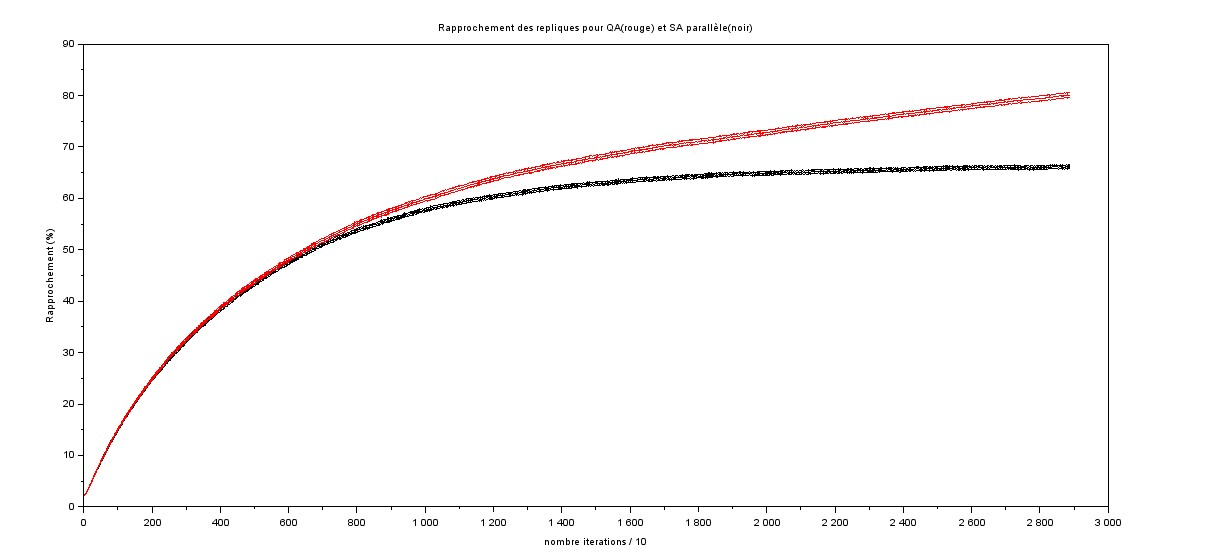
\includegraphics[scale=0.3]{rapprochement.jpg}
	\caption{Rapprochement des répliques pour QA et SA parallèle sur pr76}
	\end{center}
	\end{figure}

		Le rapprochement sur les recuits simulés en parallèle est uniquement dû à la convergence des répliques vers le minimum global. L'écart entre les deux courbes illustre le rôle du terme cinétique dans l'hamiltonien. C'est en quelque sorte le pari lancé par le recuit quantique : rapprocher les répliques entre elles pour explorer l'espace convexe constitué par ces routes.
		
		\vspace{1cm}
		La comparaison des deux recuits se fera pour des probabilités d'acceptation identiques afin de ne pas influencer le résultat final de l'expérience. Pour cela, on prend $T_{SA} = T_{QA} \times P $ où P est le nombre de répliques. La température est réglée par notre paramétreur, de même que $\Gamma$. Le nombre de répliques idéal est utilisé. La courbe obtenue sur l'évolution des énergies est celle de la figure~\ref{QASA}. Il faut zoomer sur les dernières évaluations du recuit.
		
	\begin{figure}[ht]
	
	\begin{center}
	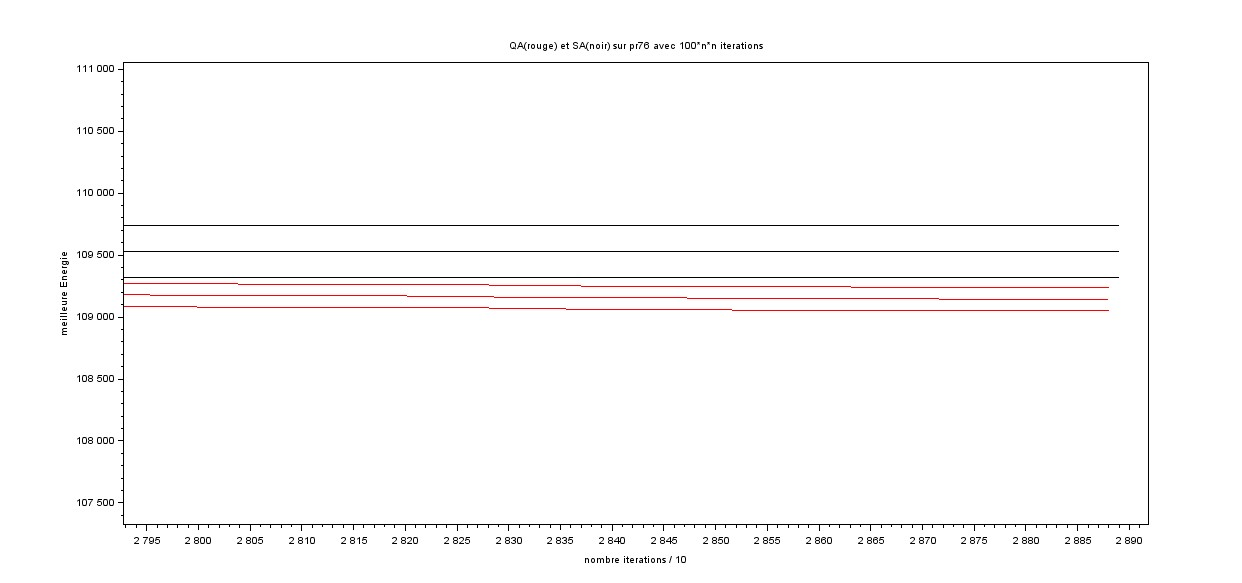
\includegraphics[scale=0.25]{zoom_pr76.jpg}
	\caption{Meilleures Energies des dernières itérations des expériences SA et QA}
	\label{fin}

	\end{center}
		
	\end{figure}
	
		Le recuit quantique obtient une énergie finale inférieure à celle du recuit simulé. De plus, on voit sur la figure~\ref{fin} que les intervalles de confiance à 95\% ne se chevauchent pas, ce qui donne un avantage considérable au recuit quantique.
		
		Une autre comparaison a été effectuée avec un autre benchmark à 58 noeuds (figure~\ref{comparaison}).
	
	\begin{figure}[!ht]
		
	\begin{center}
	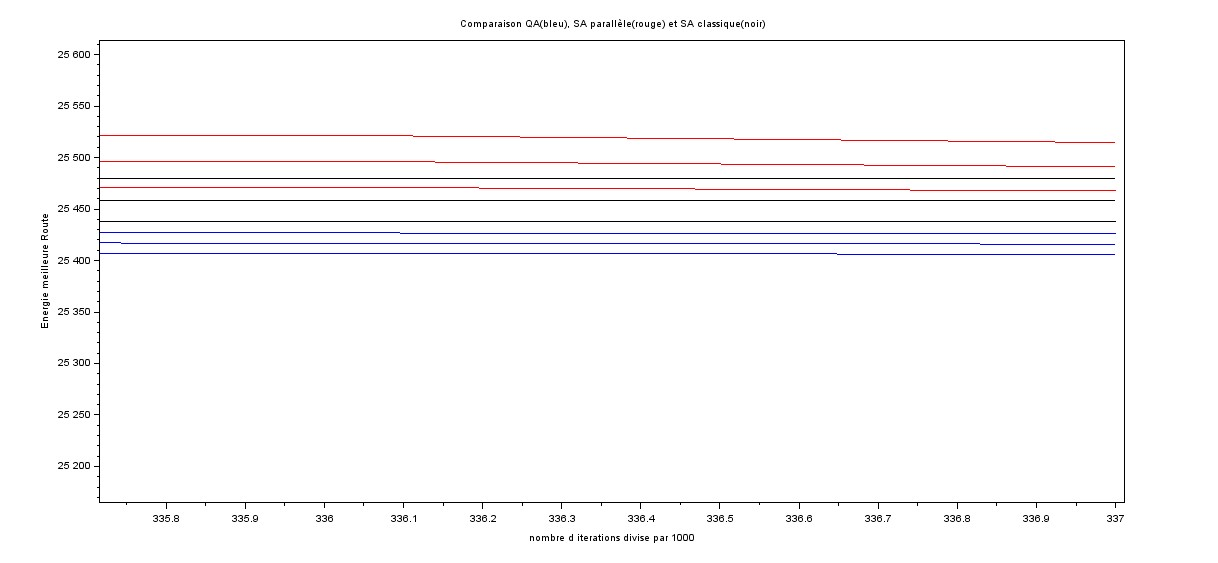
\includegraphics[scale=0.25]{brazil58_zoom.jpg}
	\caption{Evolution de l'énergie sur SA, SA parallèle et QA en fin de recuit}
	\label{comparaison}
	\end{center}
	\end{figure}

	
		Il est interessant de voir que tout l'intérêt du recuit quantique repose dans l'ajout du terme cinétique : en effet, SA parallèle obtient des résultats moins bons que SA alors que le recuit quantique est avantageux comparé à ces deux algorithmes.
		

\clearpage	
\section*{Conclusion}

\clearpage	
\listoffigures
\listofalgorithms
\bibliography{thebibliography}
\end{document}
